\documentclass[12pt]{article}
% \usepackage[margin=1in]{geometry}
\usepackage{graphicx}
\usepackage{amsmath}
\usepackage[]{algorithm2e}
% \usepackage[table]{xcolor}          % table alternate background shading
% \usepackage[LGRgreek]{mathastext}   % Dirty solution: change all math font to upright
\usepackage[style=alphabetic]{biblatex}

\newcommand{\norm}[1]{\left\lVert #1 \right\rVert}

\addbibresource{rec-notes.bib}

\title{Recommender System Notes}
\author{Tiangang Chen, Mengqiao Zhang}
\begin{document}
\maketitle
\section{Intro}
In our project, we implemented a naive version of Twitter's preliminary recommender system \cite{wtf} for recommending who to follow. We also implemented a very simple cosine-distance based content-filtering algorithm as a complement.

These two algorithms are written in Python scripts, intended to be executed by the OS scheduler on fixed time interval. So the recommendation is not reactive immediately to user input.

This document serves to record the details of our understanding and implementation, primarily as our self-reference.

\section{Content Filtering}

We collect the following raw personal information: gender, major, and tags. The tags are predefined predicates of a person's hobbies/traits that the user may select as he/she sees fit.

We model the tags as a boolean vector with dimension of number of tags available.

The rank/similarity score between two users $u$ and $v$ is calculated as follows:

\[\frac{u \cdot v}{\norm{u}_2 \norm{v}}_2\]

Which is readily available via \texttt{1 - scipy.spatial.distance.cosine(u,v)}.

\section{Collaborative Filtering}

The following illustrates an overview of the algorithm described in \cite{wtf}.

\begin{figure}[h]
\begin{center}
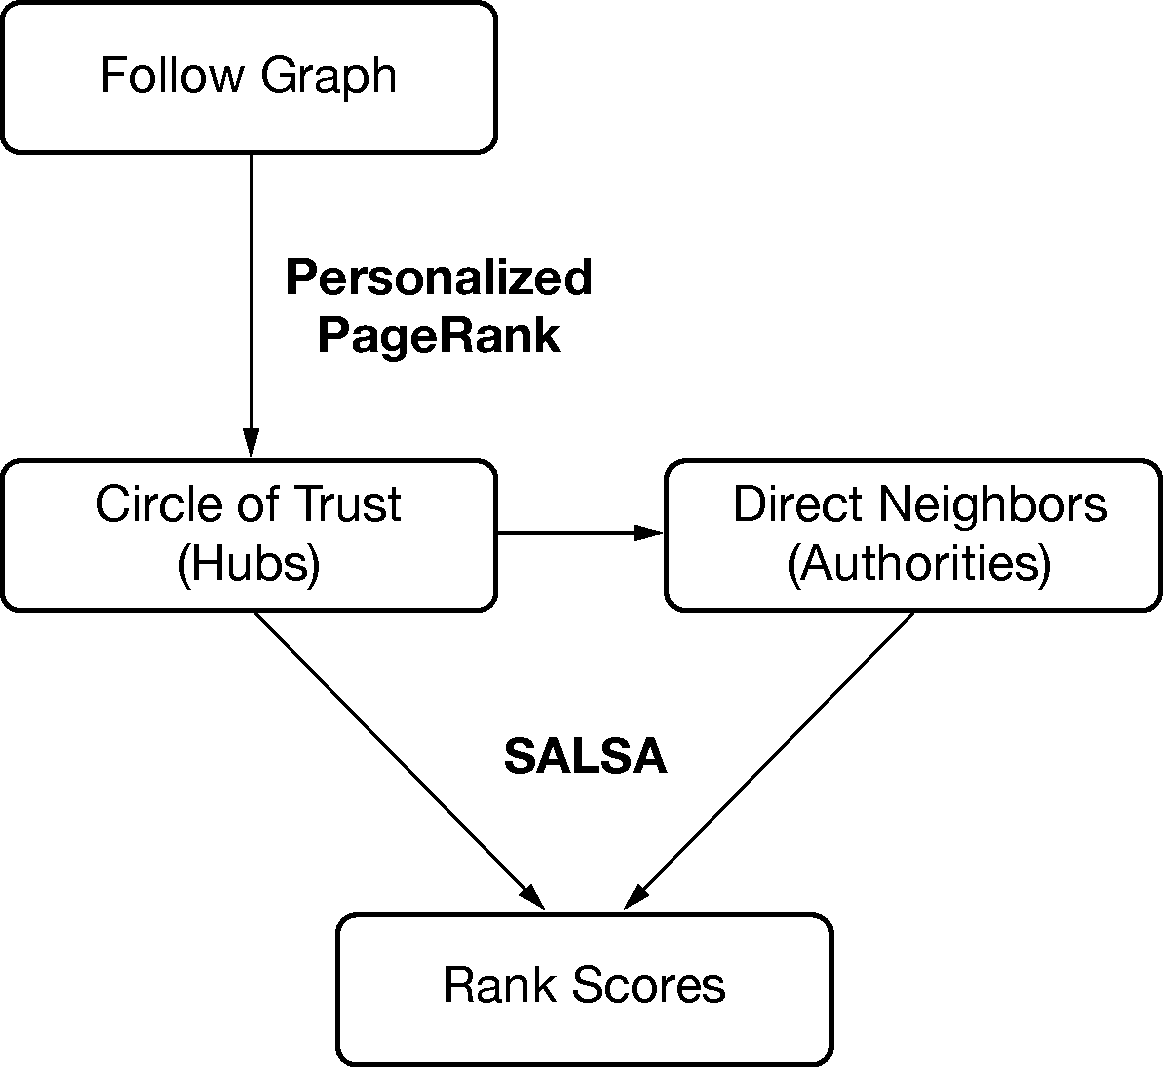
\includegraphics[width=0.5\textwidth]{wtf-algorithm}
\caption{overview of the algorithm}
\end{center}
\end{figure}

\subsection{PageRank}

The setup for PageRank \cite{pagerank} is as follows: let $u$ be a web page, $F_u$ be the set of pages that $u$ points to, and $B_u$ be the set of pages that points to $u$. Let $N_u = |F_u|$, which is the number of links originating from $u$. $c$ is the factor for normalization.

The simplified PageRank:

\[R(u) = c \sum_{v \in B_u}{\frac{R(v)}{N_v}}\]

\[R = cAR\]

Where $A$ is the matrix representation of the graph. $A_{u,v} = \frac{1}{N_u}$ if there is an edge from $u$ to $v$, otherwise $0$.

Simplified PageRank suffers from ``rank sink'' when we encounter situation similar to: two pages pointing only to each other, then some other page points to one of them. Then the rank will accumulate in the two pages but never distribute.

The improved PageRank includes a source of rank $E(u)$:

\[R(u) = c \sum_{v \in B_u}{\frac{R(v)}{N_v} + cE(u)}\]

\[R=c(AR+E)\]

We aim to maximize $c$ and keep $\norm{R}_1 = 1$. Because $\norm{R}_1 = 1$, we can rewrite $R = c(A+E \cdot 1)R$ where $1$ is a vector of all ones. The introduction of vector $E$ remedies the rank sink. Generally, we can populate $E$ with uniform value. By giving $E$ some bias we can obtain a ``personalized'' ranking focusing on a particular webpage.

We simply implement PageRank as follows, identical to the original \cite{pagerank} algorithm:

\begin{center}
\begin{algorithm}[h!]
\KwData{$R$ the rank vector\;
$A$ matrix representation of the graph\;
$E$ the initialization vector\;
$\epsilon$ convergence limit\;}
initialize: $R_0 \gets E$ \;
 \While{$\delta > \epsilon$}{
  $R_{i+1} \gets AR_i$\;
  $d \gets \norm{R_i}_1 - \norm{R_{i+1}}_1$\;
  $R_{i+1} \gets R_{i+1} + dE$\;
  $\delta \gets \norm{R_{i+1} - R_i}_1$\;
 }
 \caption{PageRank}
\end{algorithm}
\end{center}

\subsection{SALSA}

SALSA \cite{salsa} operates on a bipartite graph, traversing while assigning scores to nodes on both sides. The two sets of nodes are called hubs and authorities. In our case, the set of hub nodes consist of top results from personalized PageRank for a user, called the ``circle of trust'', and the set of authority nodes consist of direct (one degree) neighbors of those hub nodes.

We set up SALSA as follows: initially we have a collection (set) of pages, denoted by $\mathcal{C}$, edges are directed in this collection. Now we convert $\mathcal{C}$ to an undirected bipartite $G = (V_h, V_a, E)$, where

\[V_h = \{ s_h | s \in \mathcal{C}, \; \mathrm{outDegree(s)} > 0 \}\]
\[V_a = \{ s_a | s \in \mathcal{C}, \; \mathrm{inDegree(s)} > 0 \}\]
\[E = \{ (s_h, r_a) | s \rightarrow r \; in \; \mathcal{C} \}\]

So a page with both nonzero in-degree and out-degree will appear on both sides of the bipartite. Our $\mathcal{C}$ consists of the previously mentioned ``circle of trust'' and the nodes that they point to, which is naturally a bipartite.

Now we perform two distinct random walks on $G$. The two walks start from opposite side of the bipartite, traversing two edges in each iteration. So they will end up at the same side where they started. This process is represented as two Markov chains. The transition matrices are defined as follows:

\[h_{i,j} = \sum_{\{k | (i_h, k_a), (j_h, k_a) \in G\}}{\frac{1}{deg(i_h)} \cdot \frac{1}{deg(k_a)}}\]
\[a_{i,j} = \sum_{\{k | (k_h, i_a), (k_h, j_a) \in G\}}{\frac{1}{deg(i_a)} \cdot \frac{1}{deg(k_h)}}\]

Our goal is to find the pricipal eigenvectors of the hub and autority matrix, which are eigenvectors with eigenvalues of the largest magnitude. It has been argued in \cite{salsa} that such eigenvalue/eigenvector exists and is unique (has multiplicity of one). The values within are the assigned scores for the hub and authority nodes. Higher values stand for higher probability of the random walk ends up at the nodes.

\printbibliography
\end{document}
